% to choose your degree
% please un-comment just one of the following
\documentclass[bsc,frontabs,twoside,singlespacing,parskip,deptreport]{infthesis}     % for BSc, BEng etc.
% \documentclass[minf,frontabs,twoside,singlespacing,parskip,deptreport]{infthesis}  % for MInf

\usepackage{url}
\usepackage{hyperref}
\usepackage{mathtools}
\usepackage{makecell}
\usepackage{graphicx}
\usepackage{wrapfig}
\usepackage{lipsum}

\begin{document}

\title{A User-Space File-system based on Key-Value stores}

\author{Afshin Sabahi Khosroshahi}

% to choose your course
% please un-comment just one of the following
%\course{Artificial Intelligence and Computer Science}
%\course{Artificial Intelligence and Software Engineering}
%\course{Artificial Intelligence and Mathematics}
%\course{Artificial Intelligence and Psychology }   
%\course{Artificial Intelligence with Psychology }   
%\course{Linguistics and Artificial Intelligence}    
\course{Computer Science}
%\course{Software Engineering}
%\course{Computer Science and Electronics}    
%\course{Electronics and Software Engineering}    
%\course{Computer Science and Management Science}    
%\course{Computer Science and Mathematics}
%\course{Computer Science and Physics}  
%\course{Computer Science and Statistics}    

% to choose your report type
% please un-comment just one of the following
%\project{Undergraduate Dissertation} % CS&E, E&SE, AI&L
%\project{Undergraduate Thesis} % AI%Psy
\project{4th Year Project Report}

\date{\today}

\abstract{
Recent storage device hardware trends enables a new approach to the design of file systems.
Advances in Non-Volatile Memory(NVM) technologies, are blurring the line between storage and memory.
These NVM devices support load/store operations and provide new APIs. Emerging storage technologies such as KV SSDs \cite{samsung_kv_ssd} opens a new path way to how file systems can be implemented. User space drivers for  these NVMe devices allows applications to directly access without the kernel overhead \cite{spdk}. This paper introduces the design and implementation of a user space POSIX compliant file system using key-value stores. The system is designed to provide efficient and scalable access to both large and small files.
}


\maketitle

\newcommand\tab[1][2cm]{\hspace*{#1}}
\section*{Decleration}
I declare that this thesis was composed by myself, that the work contained herein is
my own except where explicitly stated otherwise in the text, and that this work has not
been submitted for any other degree or professional qualification except as specified.
\\
\tab \tab \tab \tab --Afshin Sabahi Khosroshahi

\section*{Acknowledgements}
%Acknowledgements go here. 
I would like to thank my parents, who have supported me throughout entire process, by keeping me harmonious and providing their invaluable guidance and kindness. I will be grateful forever for your love.
\\ I would like to also express my gratitude to my supervisor Pramod Bhatotia for the useful comments, remarks through the learning process of this project.

\tableofcontents

\chapter{Introduction}
% covering motivation, project overview and key contributions
\section{Motivation}
Users with ever-increasing data storage requirements use two solutions: file systems and databases. File systems are designed to store large files such as movies and VM images. Users expect to access files sequentially at close to disk throughput, requiring file data to be stored on disk with minimal fragmentation. Databases, how-ever, store large numbers of comparatively small tuples, all indexed so that lookups and scans are efficient. Additionally, transactional semantics are a must for applications to maintain consistent relationships between the large numbers of tuples that databases support.Today, users must choose between file systems and databases.  If program data does not precisely fit one of these two options — or requires both — then developers have to carefully consider the workload to decide which trade-off will hurt performance the least. Applications that manage both kinds of data can do no better than to manage data in two separate stores. For example, training deep NNs with millions of images, would require to cache large data sets into RAM for fast access. RAM is volatile and non persistent. An approach to provide these specialised complex workloads with direct access to a fast persistent memory storage device such as NVMe, can accelerate and simplify their code complexity. \cite{pmemkv}

The project overview and design goals are described in section \ref{proj_overview}. 

\section{Key contributions}
This project was initially titled as implementing a user space file system using Intel SPDK\cite{spdk}. After much research and discussing possible approaches to tackling the problem with my supervisor, I decided on implementing a file system based on key value stores. These are the key contributions I have done to finish this project:
\begin{itemize}
	\item Research emerging storage devices, such as NVMe\cite{wiki:NVM}.
	\item Research emerging new software APIs, such as SPDK\cite{spdk}, PMDK\cite{pmdk}
	\item Research possible storage engines such as Key value stores which are optimised for persistent memory devices. e.g. RocksDB\cite{rocksdb}, LevelDB\cite{leveldb}, Samsung KVSSD\cite{samsung_kv_ssd}.
	\item Learn building a C++ shared library, CMake build system.
	\item Learn and research POSIX\cite{POSIX} file API standards and specifications.
	\item Learn, understand user space file systems and their limitations.
	\item Design a file system layout which is efficient for a key value store.
	\item Develop solutions for limitations enforced by key value storage engines, e.g. storing binary data, appending to stored data and serialisation.
	\item Develop the file system, while complying with POSIX standard requirements.
	\item Evaluate the overhead produced by my file system against native key value store performance.
\end{itemize}

\chapter{Background}
%necessary background material
\section{Essential Background on Persistent memory}
The terms persistent memory and storage class memory are synonymous, describing media with byte-addressable, load/store memory access, but with the persistence properties of storage.
The article Persistent Memory Programming \cite{PMP} explains in details what are persistent memories and describes available software APIs to access these storage devices.

\section{Essential background on User space NVMe drivers}
User space NVM Express drivers provide 6x performance gains over kernel NVM Express drivers. The article "A Development Kit to Build High Performance Storage Applications" \cite{spdk_ieee} explains how this is achieved. The result is a ongoing project called Intel SPDK\cite{spdk}, a user space, polled-mode, asynchronous, lockless NVMe driver. This provides zero-copy, highly parallel access directly to an SSD from a user space application.
\\ After careful research into this project, in order to find a way to build a file system, I found out that key value stores such as RocksDB\cite{rocksdb} can be configured to run in this environment. SPDK provides a flat file system called BlobFS(Blobstore Filesystem). This file system has many limitations and still under development. It has been tested to support RocksDB, but still very immature. However more research into available persistent storage engine APIs, I found experimental tools such as pmemkv\cite{pmemkv} and Samsung's new KVSSDs \cite{samsung_kv_ssd}. This convinced me to design my project based on key value stores. 
\\
However since these software APIs require actual hardware, and are currently experimental, I wouldn't be able to use them for my development. So I used actual stable key value store databases. e.g. LevelDB and RocksDB.
\\
The core interface that these databases provide, are mostly identical. Put and Get operations are for loads and stores. Iterators allow for range scans over key value pairs. Hence I have designed my system based on this basic core functionalities for easy transition between key value store engines.

\section{Essential background on Key value databases}
I mentioned LevelDB\cite{leveldb} and RocksDB\cite{rocksdb} in the earlier section. These are high performance embedded databases for key value data, based on Log structured merge trees. 
\cite{LSM_Trees}
 RocksDB is a fork of LevelDB by Facebook optimized to exploit many central processing unit (CPU) cores, and make efficient use of fast storage, such as solid-state drives (SSD), for input/output (I/O) bound workloads.
 
\chapter{Overview} \label{proj_overview}
%system design goals. interface overview, and basic functioning
The design goal of this project is to provide user space implementation of POSIX file APIs using key value stores. The project aims at accelerating single application workloads, to fully utilise emerging storage devices capabilities. 
\\ I present an API named {\bf kvfs} (short for key-value file-system) with modularised design and capable of using any key value store implementation as storage engine.
\\ {\bf kvfs} is a C++ shared library developed using ISO C++ standard template library and C POSIX library.
The target supported operating system is currently Linux. Under current implementation of {\bf kvfs} applications can directly link to the library to perform storage operations.
\\ The library is intended for applications that want to create and manage a file system on persistent memory without the kernel overhead. The interfaces in this library are modelled after the corresponding POSIX interfaces for file management. Using interfaces modelled on POSIX allows for easier transition for application developers.

\section{kvfs storage engines}
{\bf kvfs} provides two storage engines that conform to the same common API {\ref{kvstore_abstract}. Most key value store engines can be used with {\bf kvfs} implementing the common API 
\ref{kvstore_abstract}. 
\\ RocksDB and LevelDB are currently available for use. 
\section{Requirements}
Currently {\bf kvfs} only supports a debian based linux, such as Ubuntu. I have developed this project on a Ubuntu 18.04 system. An script at {\tt kvfs/install\_dependecies.sh} can be used to install the requirements, for debian system only.
\begin{itemize}
   \item {\tt build-essentials}
	\item {\tt cmake >= v3.9}
	\item {\tt gcc, g++ >= v8.0}
	\item {\tt libsnappy-dev  \# optional, used for LevelDB}
\end{itemize}
\section{Building}
{\bf kvfs}-specific cmake variables:
\begin{itemize}
	\item {\tt BuildWithTests = ON \# enables kvfs tests builds}
	\item {\tt BuildWithRocksDB = OFF \# changes kvfs key value store engine to use RocksDB}
	\item {\tt BuildWithLevelDB = ON \# By default kvfs uses LevelDB as storage engine. Much more compact library and builds faster than RocksDB}
	\item {\tt BuildWithThreadSafety = OFF \# options to enable synchronisation using mutexs}
\end{itemize}
Sample steps to build {\bf kvfs} with LevelDB are included in the {\tt kvfs/Readme.md} file:
\begin{itemize}
	\item {\tt mkdir build}
	\item {\tt cd build}
	\item {\tt cmake DCMAKE\_BUILD\_TYPE=Release ../}
	\item {\tt cmake --build . -- -j 4}
\end{itemize}

\section{kvfs API}
{\bf kvfs} API provides a generic interface for users to perform file system operations on different types of key value stores. The main entry is at 
{\tt kvfs/include/kvfs/}.
The interface implementation details and file system limitations are described in section \ref{kvfs_library}.
\subsection{Supported interfaces}
The following interfaces are provided by {\bf kvfs} through {\tt FS} interface class.
\subsubsection{Access Management}
{\tt
	int Access(const char *filename, int how)
	\\
	int ChMod(const char *filename, mode\_t mode)
	\\
	int ChDir(const char *path)
}
\subsubsection{File Creation and Deletion}
{\tt
	int Open(const char *filename, int flags, mode\_t mode)
	\\
	int Close(int filedes)
	\\
	int Link(const char *oldname, const char *newname)
	\\
	int UnLink(const char *filename)
	\\
	int Remove(const char *filename)
}
\\
\subsubsection{open/creat Flags Support}
{\tt
	O\_APPEND \\ \tab This flag is supported. Makes writes to files append only.
	\\
	O\_ACCMODE \\ \tab This flag is checked to be a valid of types: \\ \tab \tab (O\_RDONLY, O\_WRONLY, O\_RDWR)
	\\
	O\_CREAT \\ \tab Supported, either creates a new file or opens and existing file
	\\
	O\_EXCL \\ \tab Supported, creates a new file if and only if it does not exist, otherwise throws error.
\\
	O\_ASYNC
	\\ \tab This flag is ignored.
\\
O\_CLOEXEC
	\\ \tab This flag is always set.
\\
O\_DIRECT
	\\ \tab	This flag is ignored.
\\
O\_NOATIME
	\\ \tab Is supported. Does not modify file's time stamps.
\\
O\_NONBLOCK or O\_NDELAY
	\\ \tab These flags are ignored.
\\
O\_NOCTTY
	\\ \tab Not supported.
\\
O\_PATH
	\\ \tab Sockets are not supported.
\\
O\_SYNC, O\_DSYNC
	\\ \tab These flags are ignored. Writes depend on the storage engine. Writes to persistent memories however are always synchronous.
}
\subsubsection{File Naming}
{\bf kvfs} does not support renaming files between different instances of kvfs file systems.\\
{\tt
	int Rename(const char *oldname, const char *newname)
}
\subsubsection{File I/O}
{\tt
	ssize\_t Read(int filedes, void *buffer, size\_t size)
	\\
	ssize\_t PRead(int filedes, void *buffer, size\_t size, off\_t offset)
	\\
	ssize\_t Write(int filedes, const void *buffer, size\_t size)
	\\
	ssize\_t PWrite(int filedes, const void *buffer, size\_t size, off\_t offset)
}
\subsubsection{Offset management}
{\tt
	off\_t LSeek(int filedes, off\_t offset, int whence)
	\\
	int Truncate(const char *filename, off\_t length)
}
\subsubsection{File Status}
{\tt
	int Stat(const char *filename, kvfs\_stat *buf)
}
\subsubsection{Directory Management}
{\tt 
	int MkDir(const char *filename, mode\_t mode)
\\
	kvfsDIR *OpenDir(const char *path)
\\
	kvfs\_dirent *ReadDir(kvfsDIR *dirstream)
	\\
	int CloseDir(kvfsDIR *dirstream)
\\	
	int RmDir(const char *filename)
\\
	char *GetCWD(char *buffer, size\_t size)
	\\
	std::string GetCurrentDirName()
}
\subsubsection{Symbolic Link Management}
{\tt
	int SymLink(const char *path1, const char *path2)
	\\
	ssize\_t ReadLink(const char *filename, char *buffer, size\_t size)
}
\subsubsection{Timestamp Management}
{\tt
	int UTime(const char *filename, const struct utimbuf *times)
}
\subsubsection{Special files}
For now only S\_IFREG file type is supported.\\
{\tt int Mknod(const char *filename, mode\_t mode, dev\_t dev)}
\subsubsection{Sync management}
For invoking sync on a key value store engine, whose writes are asynchronous. These two functions are equals.
{\tt
\\
	void Sync()
	\\
	 int FSync(int filedes)
}
\subsubsection{kvfs special functions}
{\tt
	int UnMount() override;
}

\chapter{Design and implementation}
%design details
%The design goal of {\bf kvfs} is to provide a single storage implementation that handles different workloads and supports full file system operations with minimal overhead. First, I present a storage system capable of supporting file system workloads using key value stores. Applications can use {\bf kvfs} to perform POSIX I/O operations.  Next I introduce {\bf kvfs} architecture, then discuss the details of the API's design pattern.

\section{kvfs software architecture overview}
Figure \ref{fig:kvfs_architecture} shows the current software system's architecture of {\bf kvfs}.  {\bf kvfs} provides a POSIX-compliant file system API for applications. A user application will link to {\bf kvfs} API and file system requests are went through this API.
{\bf kvfs} translates the requests into key value store operations. 
\begin{figure}[h]
	\centering
	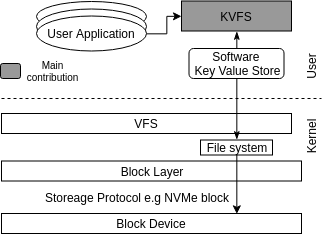
\includegraphics[scale=0.6]{diagrams/kvfs_architecture_current.png}
	\caption{{\bf kvfs} architecture}
	 \label{fig:kvfs_architecture}
\end{figure}

%\chapter{Implementation}
%%implementation details covering lowlevel details

\section{File system library} \label{kvfs_library}
The main public library is called {\bf kvfs}. There are two public header files,  {\tt fs.h} and {\tt kvfs.h}. 
\begin{itemize}
	\item {\tt fs.h} contains an abstract class called {\tt FS}.
	\item {\tt kvfs.h} contains an implementation of this interface, called {\tt KVFS}.
\end{itemize}
The reason for this approach is to be able to protect actual methods implementations and also provide the ability to have a shared instance of {\bf kvfs} within an application. This allows for multi threaded usage of {\bf kvfs}. Thread safety is available as an option in the CMake configurations of the the project, mutex locking overhead should be expected when this option is turned on.\\
Currently {\bf kvfs} can only be opened/initialised by one process only, possibly multi threaded, as this is a limitation enforced by most key-value stores.
\\
Figure \ref{fig:kvfs_fs_impl} shows the available operations to the user. These methods are mostly identical or in some cases similar to the POSIX.1-2017 ~\cite{POSIX} specifications. I have used the POSIX specification extensively for implementing this file system. {\bf kvfs} is compliant with the standard and users can expect functions to perform as they do defined by the standard. 
Please take note:
\\{\bf kvfs} is a user space file system, hence it lacks protective features of a kernel file system. Consequently POSIX ACL(Access control list) is not supported.
\\In the following sub sections, implementation details and library modules are described.

\begin{figure}[h!]
	\centering
	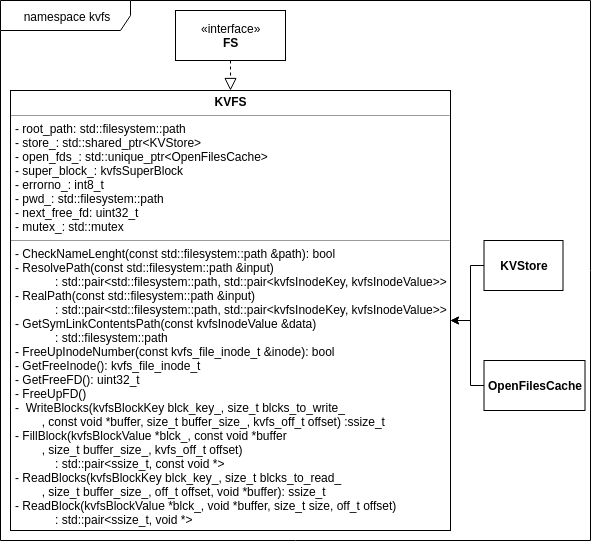
\includegraphics[scale=0.6]{diagrams/kvfs_filesystem_impl.png}
	\caption{{\bf kvfs} implementation}
	 \label{fig:kvfs_fs_impl}
\end{figure}

\subsection{kvfs file system implementation}

\subsubsection{Terminology}
{\bf kvfs} unlike traditional file systems, doesn't need to directly communicate with a storage device. It relies on the underlying key-value store to communicate with a storage device. The key-value store would use its own efficient own data structures to achieve high performance block allocation. Generally the block size for these key-value stores will be 4KiB. However since {\bf kvfs} interfaces with only key-value pairs, LBAs (logical block allocations) are overshadowed in term of these key-value pairs. For the sake of convenience, the value sizes will be referred to as block\_size of {\bf kvfs} throughout the rest of this chapter.

\subsubsection{Type definitions}
There are several types defined in {\bf kvfs}, which are used in the implementation and will be referred to respectively in this document.
These are listed in the table \ref{tab:kvfs_typedefs_table} . 
\begin{table}[h]
	\begin{center}
		\caption{{\bf kvfs} typedefs}
		\label{tab:kvfs_typedefs_table}
		\begin{tabular}{l|l|l}
		   \hline
			\textbf{Real type} & \textbf{Name} & \textbf{Description} \\
			\hline
			{\tt size\_t} & {\tt kvfs\_file\_hash\_t} & \makecell[l]{represents a type for hashes} \\
			\hline
			{\tt unsigned char} & {\tt byte} & \makecell[l]{represents arbitrary bytes} \\
			\hline
			\makecell[l]{{\tt struct dirent64} \\ or {\tt struct dirent}} & {\tt kvfs\_dirent} & \makecell[l]{dynamically represent dirent \\ based on 64bit support} \\
			\hline
			\makecell[l]{{\tt struct stat64} \\ or {\tt struct stat}} & {\tt kvfs\_stat} & \makecell[l]{dynamically represent stat \\ based on 64bit support} \\
			\hline
			\makecell[l]{{\tt ino64\_t} \\ or {\tt ino\_t}} & {\tt kvfs\_file\_inode\_t} & \makecell[l]{dynamically represent inode numbers \\ based on 64bit support} \\
			\hline
			\makecell[l]{{\tt off64\_t} \\ or {\tt off\_t}} & {\tt kvfs\_off\_t} & \makecell[l]{dynamically represent offsets \\ based on 64bit support} \\
			\hline
			\makecell[l]{{\tt \_\_kvfs\_dir\_stream}} & {\tt kvfs\_DIR} & \makecell[l]{Opaque structure for directory streams} \\
			\hline
			\end{tabular}
	\end{center}
\end{table}

\subsection{Overview} \label{overview}
A {\bf kvfs} file system is split into a series of key-value groups. These groups each have their own key structure and have distinguished prefixes. This reduces performance difficulties and reduces seek times, prefixes can act as bloom filters for the underlying key-value store. In addition the distinction, helps for identification when performing iterations and de-serializations. All fields in {\bf kvfs} are written to the key-value store relative to host's endianness. 

\subsection{Block}
{\bf kvfs} uses structures to store informations about files, file's data blocks, super block and other essential infos. There are several different structures defined for {\bf kvfs}. Each of these structures have their distinct key structure. These are described in the following sub sections \ref{structure_layouts}.
{\bf kvfs} file system maximums are described in \ref{tab:kvfs_fs_maximums}.
\begin{table}[h]
	\begin{center}
		\caption{kvfs File System Maximums}
		\label{tab:kvfs_fs_maximums}
		\begin{tabular}{l|l|l}
		   \hline
			\textbf{Item} & \textbf{Mode} & \textbf{Size} \\
			\hline
			Inodes & 64bit & $2^{64}$ \\
			& 32bit & $2^{32}$ \\
			\hline
			Blocks per file & 64bit & $2^{63}$ \\
			& 32bit & $2^{31}$ \\	
			\hline
		\end{tabular}
	\end{center}
\end{table}
A definition called {\tt KVFS\_BLOCK\_SIZE} can be set in the project's CMake configurations. 
A single typical file in {\bf kvfs} when the kvfs block size is configured as 4KiB on a 64bit host can be upto 32 ZettaBytes, since a single file can address $2^{63}$ blocks. 
Maximum number of files in the file-system is limited by the inode number.

\subsection{Layout} \label{structure_layouts}
\subsubsection{kvfs Superblock}
The superblock is a structure which records various information about the enclosing filesystem, inode counts, maintenance information, and more. The kvfs superblock is laid out in \ref{tab:kvfs_superblock_table} as follows in {\tt struct kvfsSuperBlock}. The key for super block is a constant std::string {\tt "superblock"}. 
\begin{table}[h]
	\begin{center}
		\caption{kvfs superblock}
		\label{tab:kvfs_superblock_table}
		\begin{tabular}{l|l|l}
		   \hline
			\textbf{Type} & \textbf{Name} & \textbf{Description} \\
			\hline
			{\tt uint64\_t} &  {\tt total\_inode\_count} & {Total number of used inodes} \\
			{\tt uint64\_t} & {\tt next\_free\_inode} & {First non-reserved inode} \\
			{\tt size\_t} & {\tt freed\_inodes\_count} & {Total number of freed inodes } \\
			{\tt uint64\_t} & {\tt fs\_number\_of\_mounts} & {Total count of mounts} \\
			{\tt time\_t} & {\tt fs\_creation\_time} & {Creation time in seconds} \\
			{\tt time\_t} & {\tt fs\_mount\_time} & {Mount time in seconds, since epoch} \\			
			\hline			
			\end{tabular}
	\end{center}
\end{table}

\subsubsection{kvfs Inode table}
The inode is a unique number associated to a file in {\bf kvfs}. As described in super block, free inode are tracked globally for allocations. {\bf kvfs} also handles freeing inodes when files are removed from the file system. Freed inodes are checked first for allocation before using the global free inode counter from superblock. The allocation policy will be described later in this section. Inode value structure in {\bf kvfs} is laid out in table \ref{tab:kvfs_inode_value_table}.  The definition can be found in {\tt struct kvfsInodeValue}. The inode key is defined in {\tt struct kvfsInodeKey}, which is described in table \ref{tab:kvfs_inode_key_table}.

\begin{table}[h]
	\begin{center}
		\caption{kvfs inode key structure}
		\label{tab:kvfs_inode_key_table}
		\begin{tabular}{l|l|l}
		   \hline
			\textbf{Type} & \textbf{Name} & \textbf{Description} \\
			\hline
			{\tt kvfs\_file\_inode\_t} & {\tt inode\_} & \makecell[l]{The inode number of this file's parent} \\
			\hline
			{\tt kvfs\_file\_hash\_t} & {\tt hash\_} & \makecell[l]{This file's name hash value} \\
			\hline
			\end{tabular}
	\end{center}
\end{table}

\begin{table}[h]
	\begin{center}
		\caption{kvfs inode value structure}
		\label{tab:kvfs_inode_value_table}
		\begin{tabular}{l|l|l}
		   \hline
			\textbf{Type} & \textbf{Name} & \textbf{Description} \\
			\hline
			{\tt kvfs\_dirent} &  {\tt dirent\_} & \makecell[l]{The standard POSIX structure defined in \\ {\tt dirent.h} on Linux systems which consists of \\the file's name, name length} \\
			\hline
			{\tt kvfs\_stat} & {\tt fstat\_} & \makecell[l]{The standard POSIX structure defined in \\ {\tt stat.h} on Linux systems
			which consits of \\ file attributes, permission bits and more} \\
			\hline
			{\tt kvfsInodeKey} & {\tt real\_key\_} & \makecell[l]{A pointer to the original file, if this \\ file is a hard link} \\
			\hline
			\end{tabular}
	\end{center}
\end{table}

\subsubsection{kvfs Block}
{\bf kvfs} can store a file's data in fixed size blocks defined by {\tt KVFS\_BLOCK\_SIZE}. To allow for more efficient and simpler design of blocks allocation for files, {\bf kvfs} utilises the key-value interface and implements file's blocks differently. Block key structure and value structure are laid out in the tables \ref{tab:kvfs_block_key_table}, \ref{tab:kvfs_block_value_table} respectively.

\begin{table}[h]
	\begin{center}
		\caption{kvfs block key structure}
		\label{tab:kvfs_block_key_table}
		\begin{tabular}{l|l|l}
		   \hline
			\textbf{Type} & \textbf{Name} & \textbf{Description} \\
			\hline
			{\tt kvfs\_file\_inode\_t} & {\tt inode\_} & \makecell[l]{The unique inode number of the owner \\ of this block} \\
			\hline
			{\tt kvfs\_off\_t} & {\tt block\_number\_} & \makecell[l]{This block's number} \\
			\hline
			\end{tabular}
	\end{center}
\end{table}

\begin{table}[h]
	\begin{center}
		\caption{kvfs block value structure}
		\label{tab:kvfs_block_value_table}
		\begin{tabular}{l|l|l}
		   \hline
			\textbf{Type} & \textbf{Name} & \textbf{Description} \\
			\hline
			{\tt kvfsBlockKey} & {\tt next\_block\_} & \makecell[l]{The kvfsBlockKey for the subsequent block} \\
			\hline
			{\tt size\_t} & {\tt size\_} & \makecell[l]{This block's data size} \\
			\hline
			{\tt unsigned char} & {\tt data\_} & \makecell[l]{This blocks data, an array of arbitrary bytes} \\
			\hline
			\end{tabular}
	\end{center}
\end{table}

\subsubsection{kvfs Freed Inodes}
{\bf kvfs} handles freeing inodes efficiently and stores freed inodes in arrays which are then stored in the key-value store.
As described in superblock, freed inodes count are globally tracked and this counter is used to calculate the key.  The structure used for keys and values of freed inodes are laid out in the tables \ref{tab:kvfs_freedinodes_key_table}, \ref{tab:kvfs_freedinodes_value_table} respectively.

\begin{table}[h!]
	\begin{center}
		\caption{kvfs freed inodes key structure}
		\label{tab:kvfs_freedinodes_key_table}
		\begin{tabular}{l|l|l}
		   \hline
			\textbf{Type} & \textbf{Name} & \textbf{Description} \\
			\hline
			{\tt char} & {\tt name\_} & \makecell[l]{Name prefix of freed inodes key, \\ constant {\tt "freedinodes"}} \\
			\hline
			{\tt uint64\_t} & {\tt number\_} & \makecell[l]{This freed inodes unique number} \\
			\hline
			\end{tabular}
	\end{center}
\end{table}

\begin{table}[h!]
	\begin{center}
		\caption{kvfs freed inodes value structure}
		\label{tab:kvfs_freedinodes_value_table}
		\begin{tabular}{l|l|l}
		   \hline
			\textbf{Type} & \textbf{Name} & \textbf{Description} \\
			\hline
			{\tt kvfsFreedInodesKey} & {\tt next\_key\_} & \makecell[l]{The subsequent kvfsFreedInodesKey} \\
			\hline
			{\tt uint32\_t} & {\tt count\_} & \makecell[l]{Counter for freed inodes in this block} \\
			\hline
			{\tt kvfs\_inode\_t} & {\tt inodes\_} & \makecell[l]{An array of inode numbers} \\
			\hline
			\end{tabular}
	\end{center}
\end{table}

\subsection{Inode Allocation policy}
{\bf kvfs} design recognises that data locality is a desirable quality of a filesystem. In order to reduce the total number of requests and speed up I/O in the underlying key-value store, {\bf kvfs} key structure are designed such that each each key has a specific prefix. The prefix in keys allows the underlying key-value store to sort together similar keys, adjacent keys (according to the sort order) will usually be placed in the same block. 

As described in table \ref{tab:kvfs_superblock_table}, the super block contains a global counter for next available inode number and freed inodes. When a file is created {\bf kvfs} checks the freed inodes counter to see if there are any reusable inode numbers, an inode number is taken from the last freed inodes block and the respective counters decremented. Otherwise an inode number is taken from the global counter and next available inode is incremented.

\subsection{kvfs Special inodes}
Under the current version of {\bf kvfs} the inode number "0" is a fixed allocated inode for root directory key and inode number "1" is allocated for root inode's attributes. Entries in root directory will start from 1. 
These inode numbers cannot be freed nor allocated to another file. 
The root directory name in {\bf kvfs} is defined as a single {\tt "/" }which will therefore provide a known kvfsInodeKey for {\bf kvfs} to function with. 

\subsection{Directory entries}
\begin{wrapfigure}{r}{0.6\textwidth}
	\centering
	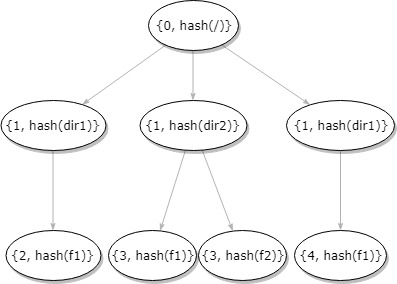
\includegraphics[scale=0.45]{diagrams/DirectoryHeirarchy.jpg}
	\caption{Sample directory heirarchy}
	 \label{fig:dir_hierarchy}
\end{wrapfigure}

In {\bf kvfs} file system, a directory is basically a file which mode type is of {\tt S\_IFDIR}. To create hierarchical structure of directories, each new entry is stored by a kvfsInodeKey as in table \ref{tab:kvfs_inode_key_table}, consisting of the file's parent inode number and the file's name hash value. A sample hierarchy is shown in figure \ref{fig:dir_hierarchy}.
\\
\\
\subsection{Reading directory entries}
When a directory is opened by function {\tt OpenDir}, a new directory stream is generated. This directory stream is an Opaque structure which holds file descriptor, and a pointer to {\tt KVStore::Iterator}. Contents of this structure are protected and cannot be queried via the user application. Upon creation of the iterator, an implicit snapshot of the key value store is taken, hence any newly added file after the directory was opened will not be retrieved.
\\ 
{\bf kvfs} utilises the scan operation provided by the key value store to implement {\tt ReadDir()} system call.  For example, when using LevelDB: 
\\ The scan operation is designed to support iterations over arbitrary key ranges, which may require searching SSTables at each level. In such a case, Bloom filters cannot help to reduce the number of SSTables to search. However in {\bf kvfs} only  needs to scan keys sharing the common prefix -- the inode number of the search directory. This can be achieved using iterator to seek to the first key containing the prefix. All other keys which are not in the desired range are ignored.
\\ This is the fastest possible approach to scanning a directory in {\bf kvfs}.
\subsection{File access and permission bits}
In {\bf kvfs} whenever a file is created, the access mode of the file shall be set to the according value of the argument in respective function(e.g. {\tt Open}, {\tt MkNod}). The file's gid (group id) shall be set to the parent's gid and uid(user id) set to the process's uid. The file's access modes can be checked via {\tt Access} function, also updated using {\tt ChMod}.
\subsection{File hard links}
Creating a hard link has the effect of giving one file multiple names (e.g. different names in different directories) all of which independently connect to the same data on the disk, none of which depends on any of the others. \cite{wiki:Hard_link}
\\ In {\bf kvfs} whenever a hard link file is created, the file's stat inode number is set to the original owner of the file. Refer to table \ref{tab:kvfs_inode_value_table}. The rest of the file's attributes are same as the original file. Hence this link can access the original file's data blocks or directory entries. The link count of both the original and new file are incremented.
\subsection{kvfs Cache}
In order to track opened files, a cache has been implemented, using an unordered map data structure. This cache is indexed by allocated file descriptors. File descriptors are abstract handlers, a non negative integer, used to refer to any UNIX file type. The cache records the opened file's inode key-value, flags which the file has been opened with as well as the current offset of this handle.
\\
Figure \ref{fig:kvfs_openfiles_cache} shows the software architecture of this cache.
\begin{figure}[h!]
	\centering
	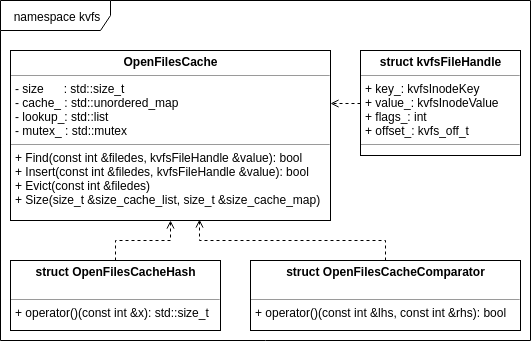
\includegraphics[scale=0.6]{diagrams/kvfs_open_files_cache.png}
	\caption{ {\bf kvfs} open files cache}
	 \label{fig:kvfs_openfiles_cache}
\end{figure}
\subsection{kvfs Error handling}
To handle errors and inform the user application of critical exceptions, a class has been developed 
using {\tt std::exceptions}. This class provides detailed error messages and corresponding error codes. The error numbers in {\bf kvfs} comply with standard POSIX system error numbers defined in {\tt error.h}. A typical usage of {\tt kvfs} shall protect function calls in try-catch blocks for correct exceptions handling. The error codes for {\bf kvfs} can be found 
in {\tt kvfs/fs/kvfs/fs\_error.h} for reference.
\\ For functions returning {\tt int}
\\{\tt 0  = success \\ -1 = failure} \\ Otherwise as defined by function return type.
\\ Error number is set in all cases of failure, Exceptions are raised to a standard Errno, values are noted.
\subsection{Limitations}
{\bf kvfs} does not support the following features:
\begin{itemize}
	\item Permissions: I only target single applications, permission control and POSIX ACL are redundant. Access and Chmod methods are provided but only if the application needs it.
	\item Extended attributes:  These are not implemented since most linux applications do not rely on it. Also its out of the scope of this project.
	\item Directory change monitoring: This is very difficult to implement correctly.Imagine writing an implementation which scales up to 10M item directories and never misrepresents a change?The demands on handling race conditions correctly are very detailed and tricky to get right in a performant and portable way. User applications should carefully change directories, to avoid errors.
\end{itemize}
\section{Key-Value store abstraction library} \label{kvstore_abstract}
This library is used to generalise and abstract {\bf kvfs}'s backing storage engine used to run  {\bf kvfs} on top of. It abstracts common and necessary operations needed for {\bf kvfs}. Common functions such as but not limited to Put and Get, Iterator API and Write-batch are implemented in this interface.  The library follows Zero copy principle, hence no overhead is produced from this abstraction. Figure \ref{fig:kvfs_KVStore_abstraction} displays this interface.
\begin{figure}[h!]
	\centering
	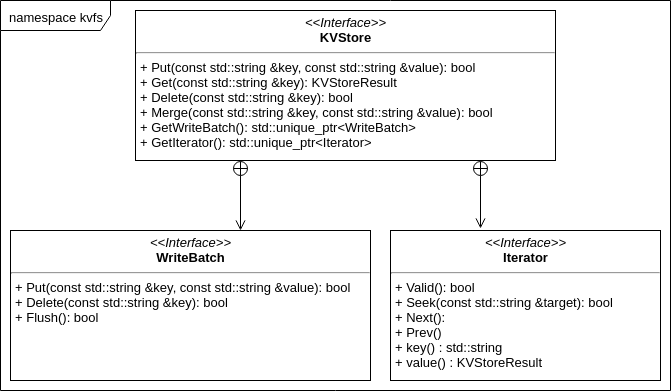
\includegraphics[scale=0.6]{diagrams/kvfs_KVStore_abstraction.png}
	\caption{ {\bf kvfs} KVStore interface}
	 \label{fig:kvfs_KVStore_abstraction}
\end{figure}
\\
There are two modules implemented for this library using LevelDB and RocksDB. Any other key value stores can be implemented following the same format. Figure \ref{fig:kvfs_kvstore_impl} shows a sample implementation format.

\begin{figure}[h!]
	\centering
	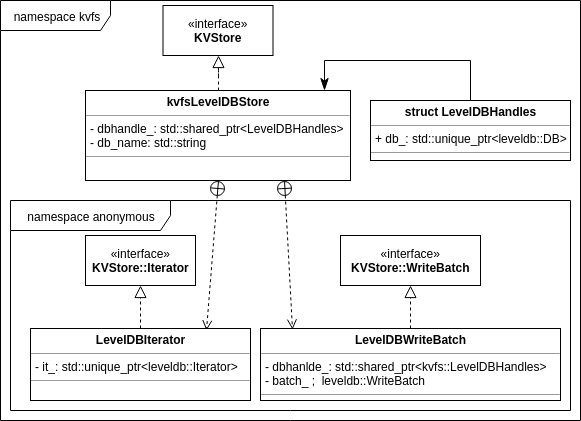
\includegraphics[scale=0.6]{diagrams/kvfs_kvstore_impl.png}
	\caption{Sample {\bf kvfs} KVStore implementation using LevelDB}
	 \label{fig:kvfs_kvstore_impl}
\end{figure}

Each module which implements the interface is composed of the following format:
\begin{itemize}
\item \textbf{Handler}: An immutable struct which encapsulates the store pointer. This struct is non copyable and takes a path name as it's argument. It handles store options and opening.
\item \textbf{KVStore}: A class which implements the {\bf kvfs}'s key-value store interface using the third party library. This class will also implement Iterator and Write-batch interfaces inside an anonymous name-space within this class.
\item \textbf{Exception}: A class which implements error messages and exception raising, which is used for this module.
\end{itemize}
\subsection{KVStore result}
The return type of values from key value stores are std::string which unfortunately gives a relatively poor memory management control.
A wrapper class \ref{fig:kvfs_kvstore_result}
\begin{wrapfigure}{r}{0.4\textwidth}
	\centering
	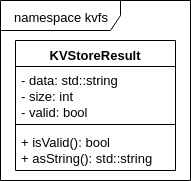
\includegraphics[scale=0.6]{diagrams/kvfs_KVStoreResult.png}
	\caption{KVStoreResult}
	 \label{fig:kvfs_kvstore_result}
\end{wrapfigure}

%, figure \ref{fig:kvfs_kvstore_result}
has been implemented around the returned string, with a few benefits: 
\begin{itemize}
\item It can represent a "not found" result, this improves efficiency and avoids throwing exceptions when key lookups are not present. 
\item This class is move only, prevents unintentional copy of the data.
\end{itemize}

\chapter{Evaluation}
%including experimental setup bechmarks and results
\section{Test system configuration}
I have developed my project in a virtual machine. The virtual machine is configured with 4 cores, 4 GiB ram. The virtual machines configuration and details are as follows: 
\tab Linux \tab Ubuntu 18.04.1, Kernel 4.18.0-17-generic
\\
\tab  CPU \tab Intel Core i7-7700HQ CPU @ 2.80GHz, 4cores - 8threads
\\
\tab DRAM \tab 4GiB DDR4 2400MHz
\\
\tab HardDisk \tab SCSI, 32GiB
\\
\tab File system \tab ext4
\\
My PC's host operating system is Windows 10 pro. The virtual machine is running on a NTFS file system. Windows is running on a Toshiba NVMe ssd. Intel premium rapid storage technology is enabled in BIOS. The drive's sequential read performance reach about 3 GB/s and writes for 1.5 GB/s.

There are three different evaluations I have implemented. The main focus is to evaluate the project based on the design goals  given in section \ref{proj_overview}.

\section{Sequential and random read/write}
I tested {\bf kvfs} against native LevelDB and ext4 file system. The overhead produced by {\bf kvfs} is very low and almost negligible. The visible overhead, is due to limitations enforced by LevelDB. This library does not allow for appending to an existing key value pair in the database, every time the value needs to be read for appends. Furthermore LevelDB only allows for writing std::strings or C style strings, which complicates when writing binary data. The data size needs to be a fixed size. C style strings end when it reaches a null value. std::string does allow for storing null bytes but converting between std::string and data structures produces some small overhead caused by memcpy.
Figures \ref{fig:seq_read}, \ref{fig:seq_write}, \ref{fig:rand_read} and \ref{fig:rand_write}  shows these benchmarks. These tests create 512 files in either random or sequential order, write binary data in those files, reads and then deletes all created files. 
{\bf kvfs} performs very well against native LevelDB considering that not only it r/ws the file's data content, but also has to update the file's timestamps and file descriptor offsets. LevelDB in the other hand is only writing either randomly or sequentially generated key value pairs. ext4 of-course has the best performance since it is running in Kernel. It is added here only for reference on how much overhead from running kv databases on a file system is produced.
\\
Ongoing projects such as Samsung's KVSSDs \cite{samsung_kv_ssd} are trying to tackle this very problem, by developing specialised firmwares for NVMe that support key value store operations natively. This would mean, there are no overheads of kernel drivers or file systems. Their benchmarks shows 10x performance gains over RocksDB instances running on a linux file system.  Their API also allows for a Zero-Copy design pattern. This suggests that my implementation could be even further enhanced, to achieve even lower overhead. However, as I mentioned in earlier chapter, these projects are still under development and were not suitable or in some cases impossible for me to use.
\begin{figure}[h!]
	\centering
	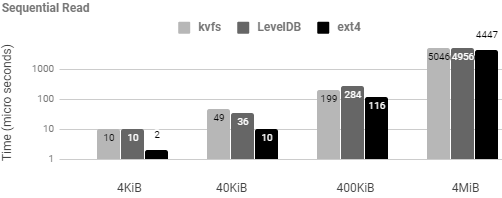
\includegraphics[scale=1]{diagrams/seq_read.png}
	\caption{Sequential read performance of 512 files}
	 \label{fig:seq_read}
\end{figure}

\begin{figure}[h!]
	\centering
	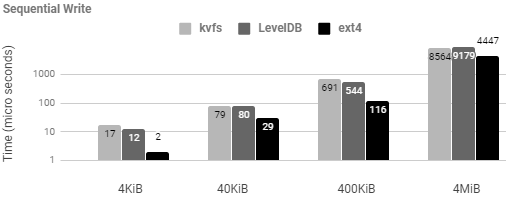
\includegraphics[scale=1]{diagrams/seq_write.png}
	\caption{Sequential write performance of 512 files}
	 \label{fig:seq_write}
\end{figure}

\begin{figure}[h!]
	\centering
	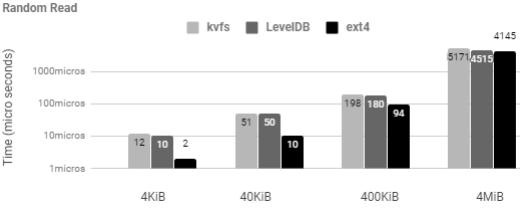
\includegraphics[scale=1]{diagrams/rand_read.png}
	\caption{Random write performance of 512 files}
	 \label{fig:rand_read}
\end{figure}
\begin{figure}[h!]
	\centering
	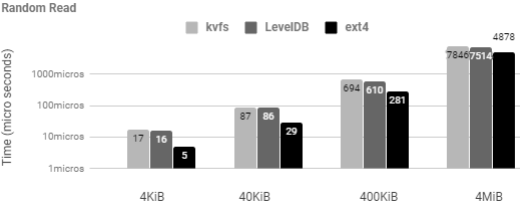
\includegraphics[scale=1]{diagrams/rand_write.png}
	\caption{Random write performance of 512 files}
	 \label{fig:rand_write}
\end{figure}

\section{Scan queries}
To test the performance of metadata intensive workload in {\bf kvfs} against ext4, I created a test to generate nested directories of 10000 files, and ran readdir on  each direcory. After calculating an average, I developed the following graph \ref{fig:readdir}. Intresingely, {bf kvfs} perform very similarly in mkdir operations. Perhaps because in {\bf kvfs} the file's metadata is stored with one operation, but for ext4 the creation of new file's is more costly. Moreover, readdir is slower in {\bf kvfs} since, entire file's attributes are returned from the kv store. However  the differenece can be argued to be the overhead of running LevelDB on ext4, as seen in previous benchmarks. Delete operations, seem very expensive, enforced by LevelDB delete performance. When a key value pair is deleted, in regards to LevelDB, entire sorted table files need to be rewritten. Consequently this is more expensive, than single deletion that takes place for ext4 files. 

\begin{figure}[h!]
	\centering
 	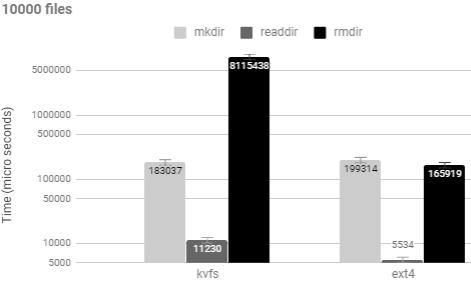
\includegraphics[scale=1]{diagrams/readdir.png}
	\caption{Creating, scanning and removing 10000 directories}
	 \label{fig:readdir}
\end{figure}

\chapter{Related work}
%explain relate work in this area
\textbf{Pmemfile} \cite{pmemfile} "is project with the goal to provide low-overhead userspace implementation of file APIs using persistent memory." This has similar goals to my project, achieves the no kernel overhead design and current applications can run with this file system using LD\_PRELOAD. However the project does not use a key value store engine, rather directly uses persistent memory programming kit \cite{pmdk}.
\\ {\bf kvfs} on the other hand, links directly with the user application, but that would mean limited compatibility. However, {\bf kvfs} can be used with self encrypting key value store engines, to support encryption. Furthermore, with the upcoming KVSSDs, {\bf kvfs} could possibly perform similarly to pmemfile project, in terms of performance.
\\ Next C++20 standard \cite{std_fs}, will standardise file APIs, therefore {\bf kvfs} could be implemented in a standard way, to support more operating system and easily integrate into user applications.

\textbf{Direct access File systems}
Kernel library modules provided by pmdk\cite{pmdk}, have been patched into most operating systems, accelerating their file system operations, by avoiding extra copies of page-cache for persistent memory devices. These prove to be very practical improvements for current most widely used file systems. However the kernel overhead, would still become a bottleneck for low latency access needs in some user application workloads. Hence, these applications could benefit from user space file system. Intel SPDK\cite{spdk} shows how kernel can become a bottleneck through their benchmarks.

\chapter{Conclusion and future work}
In this paper I presented {\bf kvfs} a user space file system based on key value stores. I developed this file system complying with POSIX standards and evaluated the file system's overhead against a native key value store engine(LevelDB). 

{\bf kvfs} with the current implementation, can have many interesting use cases. Applications that sandbox particular softwares could use {\bf kvfs} to store applications data changes.

{\bf kvfs} current implementation, updates file's attributes whenever the file is accessed. This produces an overhead which could potentially be done in the background, such that read/write operations take less even less time. A thread pool can be designed to push low priority updates to background. This thread poll would be an internal feature of {\bf kvfs}. 

A POSIX compliance benchmark test for {\bf kvfs} is for future contribution, for correct expected behaviour. This is a large project on its own and was out of scope of this project.

A system call intercept library can also be implemented for {\bf kvfs}, to seamlessly run user application on {\bf kvfs} without application modification. Another difficult task which was not possible to achieve in the time frame of this project.

% use the following and \cite{} as above if you use BibTeX
% otherwise generate bibtem entries
\bibliography{mybibfile}
\bibliographystyle{plain}

\end{document}
